\section*{Finding patterns}

Our dataset consists of the following information:

\begin{itemize}
	\setlength\itemsep{0.05em}
	\item bookingdate - Date of transaction being completed, either charged back or sent trough
	\item issuercountrycode - Country of shop
	\item txvariantcode - Type of card used
	\item bin - Grouping number similar to a batch
	\item amount - Monetary amount of the transaction
	\item currencycode - Currency used for transaction
	\item shoppercountrycode - Source country of transaction
	\item shopperinteraction - Type of transaction
	\item simple\_journal - Valid/Fraud label
	\item cardverificationcodesupplied - Card Verification Code (CVC) supplied by shopper
	\item cvcresponsecode - Response to CVC given by shopper
	\item creationdate - Date of transaction being completed
	\item accountcode - Country of shopper
	\item mail\_id - Email address of shopper
	\item ip\_id - IP address of shopper
	\item card\_id - Card number of shopper
\end{itemize}

To better understand the importance and interaction between these values, we attempted to create visualisations depicting this.

\begin{figure}
	\centering
	\caption{Transaction amount with label (Green-Settled, Red-Chargeback)}
	\label{img-amounts}
	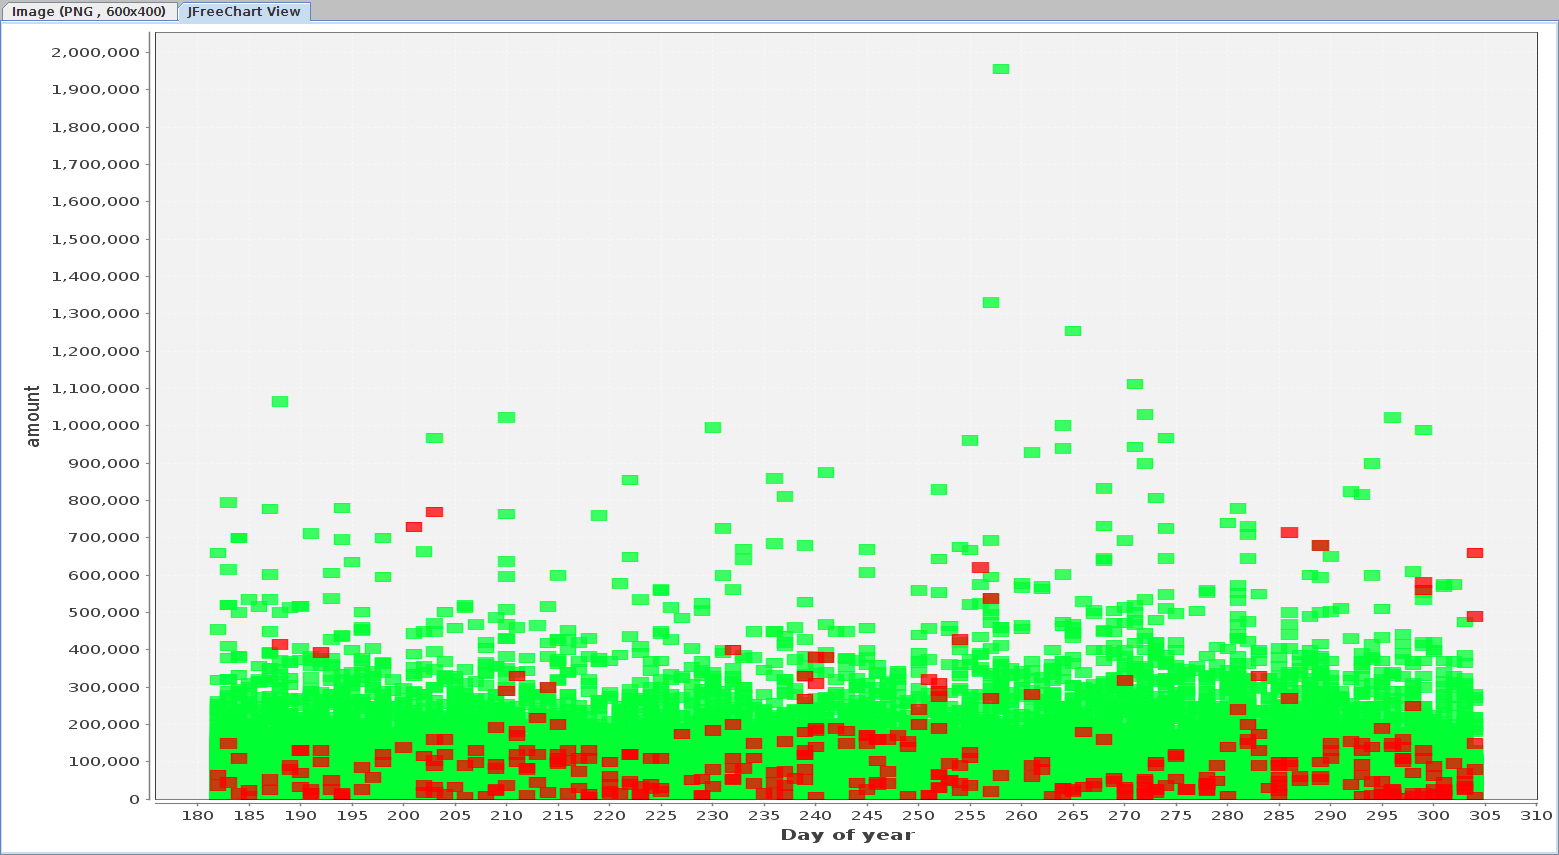
\includegraphics[width=0.6\linewidth]{amounts-transaction}
\end{figure}